\def\year{2018}\relax


\documentclass[letterpaper]{article} %DO NOT CHANGE THIS
\usepackage{aaai18}  %Required
\usepackage{times}  %Required
\usepackage{helvet}  %Required
\usepackage{courier}  %Required
\usepackage{url}  %Required
\usepackage{tikz} %Required
\usepackage{listings}
\usetikzlibrary{positioning,chains}
\usepackage{caption}
\usepackage{graphicx}  %Required
\frenchspacing  %Required
\setlength{\pdfpagewidth}{8.5in}  %Required
\setlength{\pdfpageheight}{11in}  %Required
\setcounter{secnumdepth}{0}
\usepackage{subfigure}

\lstset{
numberstyle=\small,
numbers=left,
numbersep=8pt,
frame = single,
language=Pascal,
framexleftmargin=15pt}

\begin{document}
% The file aaai.sty is the style file for AAAI Press
% proceedings, working notes, and technical reports.
%
\title{CS486 Project: Comparison of Image Recognition Algorithms}
\author{Mingkun Ni, Tianyi Zhang, Yuanhao Zhang\\
\{m8ni, y2384zha, t296zhan\}@uwaterloo.ca\\
University of Waterloo\\
Waterloo, ON, Canada\\
}
\maketitle

%%%%%%%%%. Abstract %%%%%%%%%

\section{\em{Abstract}}
\textit{Image recognition has been a popular field in Artificial Intelligence. Many real-world problems such as self-driving vehicles and medical diagnosis rely on image recognition. Researchers and programmers have came up with various neural network paradigms, such as Convolutional Neural Network(CNN), k-Nears-Neighbours, and Recurrent Neural Network(RNN). Both CNN and RNN are popular algorithms in classification problems. The main reason that RNN is chosen is due to its recurrent feature. RNN is able to discover the internal sequential relation between images. CNN is chosen since it is one of the most widely-used algorithm in the field of image recognition. Therefore, this paper will use Fashion-MNIST data set to run image recognition using CNN and RNN algorithms and compare the time complexity, memory usage, and test set accuracy of the results.}

%%%%%%%%%. Introduction %%%%%%%%%

\section{Introduction}
Catalyzed by the creation of ImageNet, the image recognition technology has advanced remarkably in recent years. The image recognition technology is fundamental to many emerging applications such as autonomous vehicles, augmented reality, medical diagnosis, etc. As the technology becomes more mature, the image recognition market is rapidly expanding. According to Markets and Markets \cite{market}, the image recognition market is estimated to grow from 15.95 billion USD in 2016 to 38.92 billion USD in 2021. The fact that the market size would be more than doubled in five years shows the significance and potential of the image recognition technology.

Recent rapid development of the image recognition technology is largely thanks to the creation of an image dataset named ImageNet. The idea was conceived by a university professor Fei-fei Li in 2006, after she had realized all of the image datasets at the time were too limited in size and variety. She thought, to make advancements in image recognition, increasing the quality and quantity of training data might help more than improving on the algorithm alone. The ImageNet dataset was born in 2009, and an annual competition using the dataset as training data was started the next year. People quickly realized that their algorithms performed better when trained on ImageNet compared to when trained on traditional image datasets. Since ImageNet contains a large sample of images of a variety of objects, it accurately reflects the performance of algorithms in the real world. In the ImageNet competition, the error rate on the test set has decreased year over year (~\ref{fig:ErrorRate}), demonstrating the steady improvements of image recognition algorithms each year. \cite{Quartz}

\begin{figure}[h!]
 \centering
  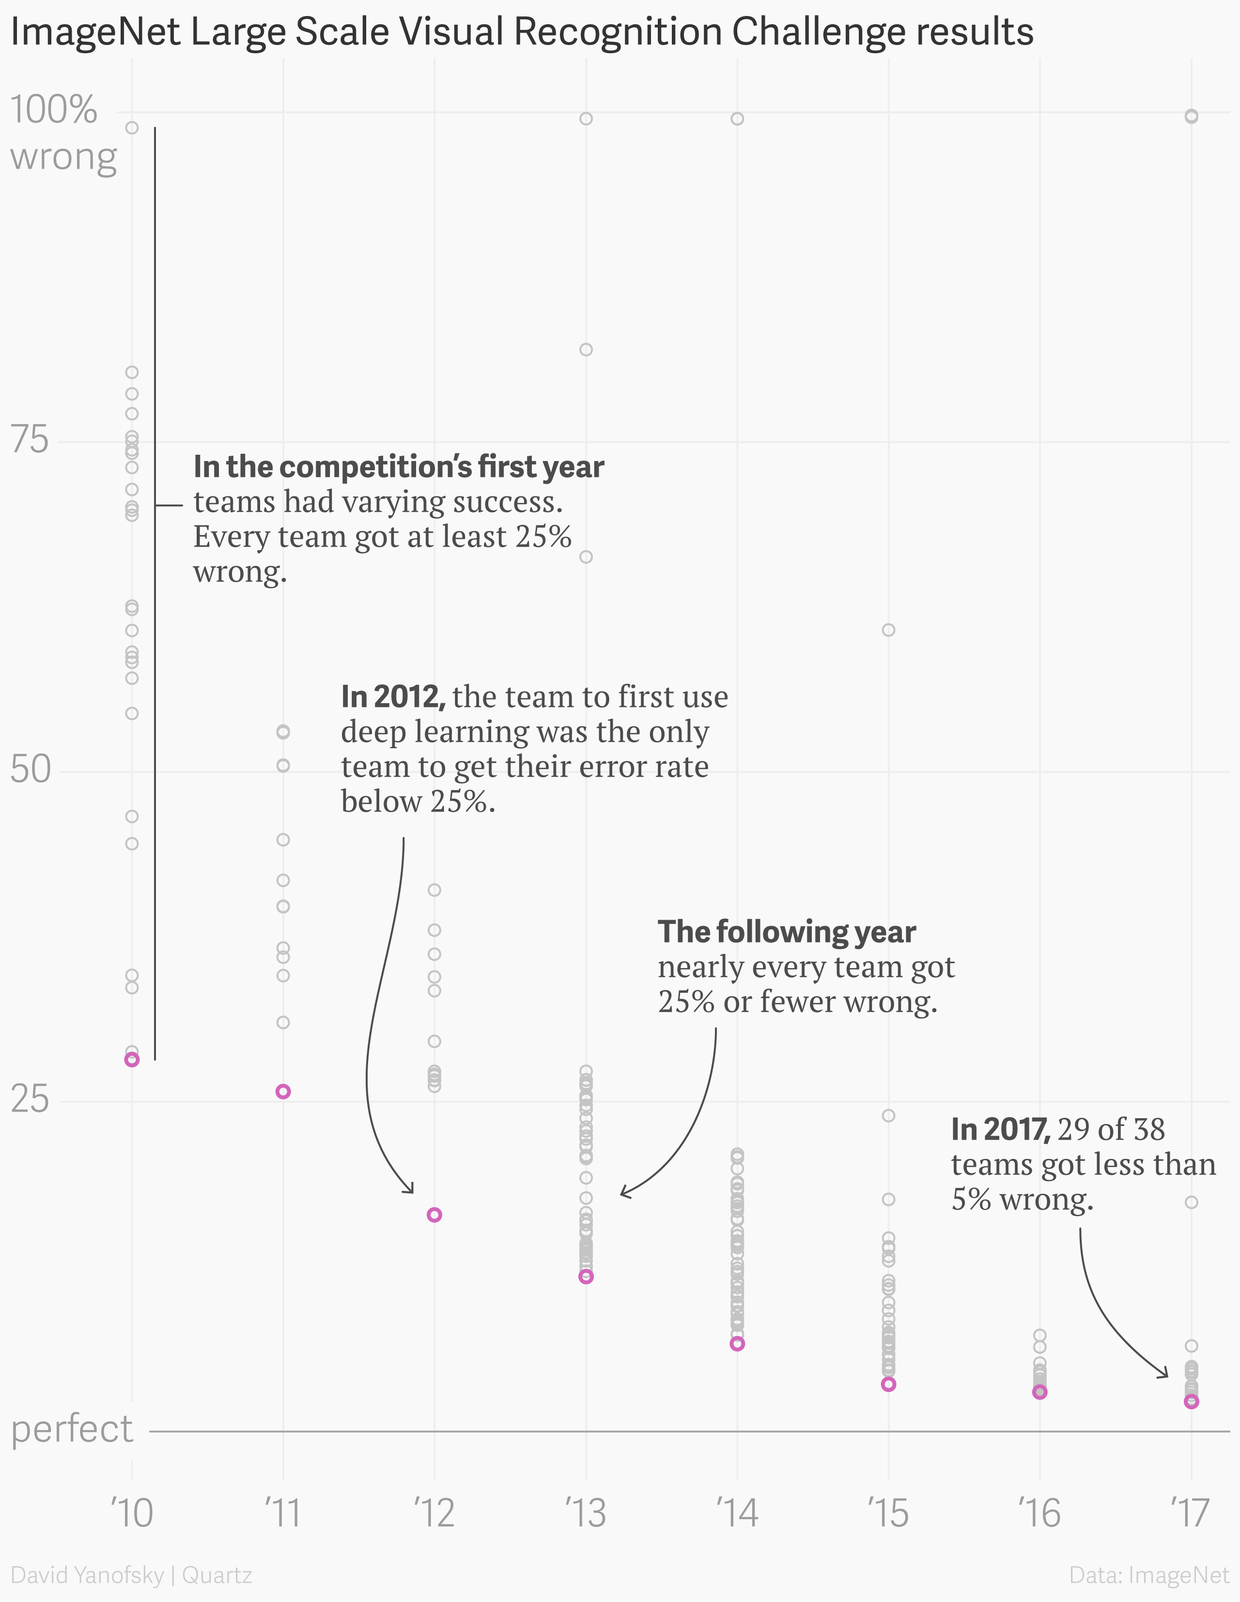
\includegraphics[width=0.5\textwidth]{intro.png}
 \caption{Error Rate of Contestants of the ImageNet Competition over the years}
 \label{fig:ErrorRate}
 \end{figure}

 Image recognition is crucial for the development of many other technologies. Autonomous driving is a booming field with heavy reliance on image recognition. Image recognition enables vehicles to understand the surrounding environment in real time, thus allowing decision making and path finding. Developing an accurate and reliable image recognition algorithm for autonomous vehicles is no small feat. In the real world, a vehicle sees all sorts of objects, and the algorithm often has to classify these objects in motion and in real time. Some of the situations a vehicle would encounter cannot be anticipated by developers in a lab. For example, Google’s self-driving car encountered possibly the weirdest road situation ever; it was stopped by a lady in a wheelchair chasing a bird on the road. \cite{birdchasing} Hence, accurate image recognition software that can identify all common objects in real time is necessary for the development of autonomous vehicles. Another field that has been gaining traction over recent years is augmented reality. Augmented reality needs quick and accurate image recognition because it superimposes information or visuals on the surroundings that users perceive. Augmented Reality has a broad range of applications including entertainment, medical applications, and military navigation and targeting. \cite{ar}

 The aim of this project is to analyze the differences between two different image recognition algorithms, Convolutional Neural Network (CNN) and Recurrent Neural Network (RNN). The analysis makes use of the dataset MNIST Fashion. The purpose of this report is to illustrate the advantages and drawbacks of the two algorithms, so a better one can be chosen for image recognition tasks.

%%%%%%%%%. Related Work %%%%%%%%%

\section{Related Work}

\cite{cios1995image,xiao2017fashion} These two papers are focusing on the general topic and the data set of image recognition using neural network. In the first paper, the proposed neural network algorithm, namely image recognition neural network, is designed to classify objects through the attributes of the images. This algorithm will take a grey-scaled image as an input and return an appropriate output to which the algorithm believes the given image matches. As an extension of the first paper, the second paper discusses the dataset that we will use in this project, named Fashion-MNIST. It contains 70,000 grey-scaled images with a size of $28 \times 28$. This paper also states that Fashion-MNIST is considered as a better dataset for problem of image recognition using neural network compared to the old MNIST data set. \\
\cite{simonyan2015very,hijazi2015using,razavian2014cnn,chen2018the,hou2016fruit,lo1995artificial}
All of these paper discuss image classification and they all manage to train the model using CNN. CNN is widely used in pattern- and image-recognition problems because they have significant benefits over other neural network techniques. In general, CNN is a good choice for image recognition because of the following properties. First, it avoids the influence of image distortion on prediction result. Second, it uses less amount of memory compared to other Neural Network algorithm. Third, CNN reduces the number of parameters dramatically; thus, training time is significantly reduced. These papers describes the basic CNN algorithm and the hidden layers to be used for a CNN algorithm. Some of the other paper discuss different applications of CNN but in the field of image recognition and demonstrate how CNN is used in the real world to solve problems. \\
\cite{le2015a,zhang2018image} This paper talking about RNN and how RNN is used to solve problems. RNN is a powerful and natural method to map a sequence of input to a sequence of output. The second paper by Zhang discusses how CNN has been widely used in the field of image recognition, but there are still limitations of the current CNN image classification paradigm. For example, CNN cannot handle images with different sizes correctly. Thus, Zhang proposed a new paradigm named Scaled Recurrent Neural Network(SRNN) that is based on RNN embedded in the current paradigm, which is able to solve leftover problems of CNN.

%%%%%%%%%. Method Description %%%%%%%%%

\section{Methodology}

Due to fast development of artificial intelligence and neural network,multiple algorithms are applied in the field of image recognition. Performance can be different based on various implementation of algorithm and training environment. This project aims to analyze the performance of two different algorithms: Convocational Neural Networks(CNN) and Recurrent Neural Network(RNN).

The data set we're using is Fashion-MNIST. Fashion-MNIST is a dataset of Zalando's article images, which consists of 60,000 examples and a test set of 10,000 examples(Han Xiao, 2017). Each image is a $28 \times 28$ grayscale image, and each has a label associated from different classes of clothing. This data set is a great selection for image recognition since it differs from MNIST which is too easy and overused and doesn't represent modern computer vision tasks. In addition, Fashion-MNIST contains a large number of training and testing sets and should be able to yield a reasonable result in term of algorithm comparison.

The first algorithm is CNN, which is a fully connected network such that each neuron in one layer is connected to all neurons in the next layer. It simplifies complex patterns derived from training data. CNN has complex architectures and it is usually constructed with four types of layers: convolutional layers, pooling layers, non-linear layers, and fully connected layers (Hijazi et. al. 2015). The purpose of the convolutional layers is generally to extract the features of the input. According to Hijazi(2015), the pooling layers are to reduce distortion and noise that may affect the process of image classification. Non-linear layers relies on activation function to match similar identification in each hidden layer. In the CNN algorithm we used in this project, the activation function used is ReLU. Lastly, the fully connected layer is the final layer that combines all the previous features and determine a target output based on the information (Hijazi et. al., 2015).

A simple and abstract mathematical formulation of CNN structure can be represented by the following:
$$x^1\rightarrow w^1 \rightarrow ... \rightarrow x^{L-1} \rightarrow w^{L-1} \rightarrow x^L \rightarrow w^L \rightarrow z$$
This simple formulation demonstrates how CNN proceed forward layer by layer. $x^1$ is the initial input and it goes through process with weight $w^1$. This process will continue until it outputs $x^{L}$. In the CNN algorithm chosen for this paper, it will be using two built-in Conv2D layer provided by Keras (Simonyan, 2015). The first Conv2D layer creates a convolutional kernel with a 3-by-3 kernel size and uses ReLU as the activation function with the input shape matching the Fashion-MNIST dataset. Following the first Conv2D layer, there is another Conv2D layer using ReLU activation function again. Then, the algorithm applies MaxPooling2D to find the max from a non-overlapping 2-by-2 block to filter out noise and distortion in the dataset while maintaining the features. A Dropout layer is used with a rate of 0.25 for the resulting neural network to have better generalization and be less likely affected by data overfitting. Then the algorithm will apply a Dense layer which is also known as a fully connected layer to connect and combine previous features and produce an output. The following is sample code for Convolutional Neural Network obtained from Xiao:
\begin{lstlisting}[columns=fullflexible, keepspaces=true, stepnumber=1]
num_classes = 10
input_shape = (1, img_rows, img_cols)
model.add(Conv2D(32, kernel_size=(3, 3),
                 activation='relu',
                 input_shape=input_shape))
model.add(Conv2D(64, (3, 3), activation='relu'))
model.add(MaxPooling2D(pool_size=(2, 2)))
model.add(Dropout(0.25))
model.add(Flatten())
model.add(Dense(128, activation='relu'))
model.add(Dropout(0.5))
model.add(Dense(num_classes, activation='softmax'))
\end{lstlisting}

CNN is considered as a good choice for image recognition problems in general. It is widely applied in related problems. Also, as stated in related work section, it has several known advantages regarding to image recognition problem, such that the influence of image distortion on prediction result will be avoided. Thus, we will evaluate its performance in this paper.

The second algorithm is RNN. RNN uses neural network to map an input sequence to an output sequence. In another word, it is designed to solve problems in term of predicting sequence. RNN is generally a good choice when dealing with classification problem. Since this report is working on image classification, RNN is chosen as one of the algorithm.

Although RNN is usually hard to train, it is able to store information in the form of activation and it is able to learn sequential data. The reason for this is that, after feeding one datapoint, it will generate a state that contains some useful information from this datapoint, and use it as input when feeding the next datapoint. Thus, neural network will understand the sequential relation between datapoints, and generate its output accordingly. Below is a mathematical representation of RNN retrived :
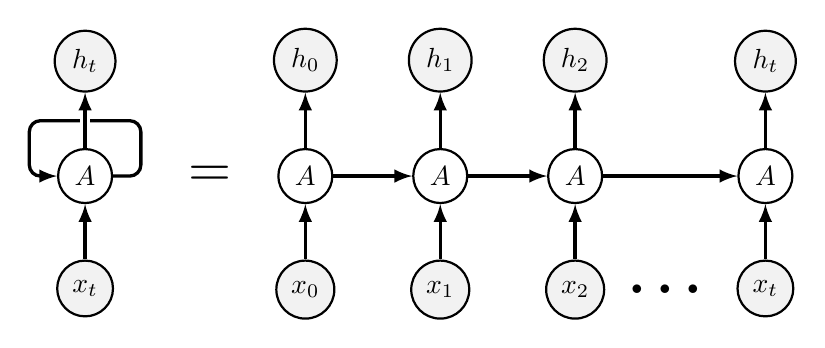
\begin{tikzpicture}[item/.style={circle,draw,thick,align=center},
itemc/.style={item,on chain,join}]
 \begin{scope}[start chain=going right,nodes=itemc,every
 join/.style={-latex,very thick},local bounding box=chain]
 \path node (A0) {$A$} node (A1) {$A$} node (A2) {$A$} node[xshift=2em] (At)
 {$A$};
 \end{scope}
 \node[left=1em of chain,scale=2] (eq) {$=$};
 \node[left=2em of eq,item] (AL) {$A$};
 \path (AL.west) ++ (-1em,2em) coordinate (aux);
 \draw[very thick,-latex,rounded corners] (AL.east) -| ++ (1em,2em) -- (aux)
 |- (AL.west);
 \foreach \X in {0,1,2,t}
 {\draw[very thick,-latex] (A\X.north) -- ++ (0,2em)
 node[above,item,fill=gray!10] (h\X) {$h_\X$};
 \draw[very thick,latex-] (A\X.south) -- ++ (0,-2em)
 node[below,item,fill=gray!10] (x\X) {$x_\X$};}
 \draw[white,line width=0.8ex] (AL.north) -- ++ (0,1.9em);
 \draw[very thick,-latex] (AL.north) -- ++ (0,2em)
 node[above,item,fill=gray!10] {$h_t$};
 \draw[very thick,latex-] (AL.south) -- ++ (0,-2em)
 node[below,item,fill=gray!10] {$x_t$};
 \path (x2) -- (xt) node[midway,scale=2,font=\bfseries] {\dots};
\end{tikzpicture}
\captionof{figure}{\textbf{Mathematical Representation of RNN}}
In the RNN algorithm chosen for this paper, it will be using one SimpleRNN Layer with 100 hidden units. It selects random normal distribution with standard deviation 0.001 as its initial weight distribution or kernel initializer and identity matrix with gain 1.0 as its recurrent initializer.Then, the algorithm will apply a Dense layer or fully-connected layer with 10 classes and activation function softmax. The following is sample code for Recurrent Neural Network:

\begin{lstlisting}[columns=fullflexible, keepspaces=true, stepnumber=1]
num_classes = 10
hidden_units = 100
model.add(SimpleRNN(hidden_units,
kernel_initializer=initializers.RandomNormal(stddev=0.001),
recurrent_initializer=initializers.Identity(gain=1.0),
activation='relu',
input_shape=x_train.shape[1:]))
model.add(Dense(num_classes))
model.add(Activation('softmax'))
\end{lstlisting}

RNN is considered in this paper because of its recurrent feature. RNN is able to discover the internal sequential relation between images. We believe that the history information or state will help us classify current image and improve recognition performance.

Two algorithm can be compared in lots of different aspects. For neural network algorithms, two aspects are relatively important indicators of performance: Accuracy and Resource Usage. For accuracy, this project will test the prediction accuracy using different values of parameters for each algorithm. For example, we will test the influence on accuracy if we change the number of training epochs each algorithm will run in test. Related result will be concluded by comparing two algorithm’s distribution of prediction accuracy. For resource usage, given the same training set and parameters, time efficiency and space efficiency will be considered and compared. For example, we will test the difference of time and memory used by running two algorithms with the same number of epochs.
We set up two test environments with Windows 10 operating system and MacOS Mojave. To test these two algorithm efficiently, we use TensorFlow with GPU support on Windows 10 and TensorFlow with CPU on MacOS while running python in bash terminal. Following are the configurations of Windows 10 and MacOS system respectively:
\begin{lstlisting}[columns=fullflexible, keepspaces=true, stepnumber=1]
System: Windows 10
CPU: i7-6700hq Memory: 8G
GPU: GTX 960m Memory: 2G
TensorFlow: tensorflow-gpu v1.14.0
CUDA: v10.0.130
cuDNN SDK: v7.6.1.34
Python: v3.7.3 64bit
\end{lstlisting}
For your information, CUDA and cuDNN SDK are softwares required to run TensorFlow with GPU support on Nividia graphic card in Windows 10 testing environment.
\begin{lstlisting}[columns=fullflexible, keepspaces=true, stepnumber=1]
System: MacOS Mojave version 10.14.4
CPU: i5-7267u Memory: 8G
GPU: Intel Iris Plus Graphics 655 Memory: 1536MB
TensorFlow: tensorflow 1.13.1
Python: 3.7.3 64bit
\end{lstlisting}

%%%%%%%%%. Result %%%%%%%%%


%%%%%%%%%. Bibliography %%%%%%%%%
\newpage
\bibliographystyle{aaai}
\bibliography{report}

\end{document}
